\documentclass[10pt]{article}
\usepackage[T1]{fontenc}
\usepackage[utf8]{inputenc}
\usepackage{lmodern}
\usepackage[a4paper,margin=24mm]{geometry}
\usepackage{amsmath,amssymb,booktabs,graphicx,array}
\usepackage{xcolor}
\definecolor{flm}{HTML}{A74C20}
\usepackage[colorlinks=true,linkcolor=flm,citecolor=flm,urlcolor=flm]{hyperref}
\usepackage{microtype}
\setlength{\parskip}{5pt}
\setlength{\parindent}{0pt}
\setlength{\emergencystretch}{2em}
\renewcommand{\arraystretch}{1.15}
\graphicspath{{figures/}}
\newcommand{\code}[1]{\texttt{\detokenize{#1}}}

% Generated by scripts/feedback_paper_data.py; do not hand-edit measurements.
\newcommand{\FeedbackErrorRows}{%
Untrained & Live & 101.48 & 92.14 & 117.09 \\
Untrained & Frozen & 101.48 & 93.91 & 117.09 \\
BPTT & Live & 7.68 & 7.26 & 16.27 \\
BPTT & Frozen & 96.41 & 93.91 & 100.50 \\
Fixed core & Live & 7.68 & 7.26 & 16.27 \\
Fixed core & Frozen & 96.41 & 93.91 & 100.50 \\
Eligibility & Live & 7.68 & 7.26 & 16.27 \\
Eligibility & Frozen & 96.41 & 93.91 & 100.50 \\
Scripted reference & Live & 7.68 & 7.26 & 16.27 \\
}
\newcommand{\FeedbackContrastRows}{%
Untrained & +0.00 & -1.77 & +0.00 \\
BPTT & -88.72 & -86.65 & -84.23 \\
Fixed core & -88.72 & -86.65 & -84.23 \\
Eligibility & -88.72 & -86.65 & -84.23 \\
}
\newcommand{\FeedbackEquivalentCount}{9}
\newcommand{\FeedbackDistinctPaths}{7}
\newcommand{\FeedbackSwitchError}{16.27}
\newcommand{\FeedbackSwitchDistance}{28.11}
\newcommand{\FeedbackPhaseOne}{10.85}
\newcommand{\FeedbackPhaseTwo}{10.91}

\hypersetup{pdftitle={FLM: Learned Choices in a Physical Feedback Loop},pdfauthor={Kuber Mehta},pdflang={en}}
\title{\textbf{FLM: Learned Choices in a Physical Feedback Loop}\\[6pt]\large Pose feedback, delayed decisions and a scripted reference}
\author{Kuber Mehta\\\href{https://flm.kuber.studio}{flm.kuber.studio}}
\date{10 September 2026 --- working research note}
\begin{document}
\maketitle
\begin{abstract}
We connect existing 256-neuron sensory-choice networks to a physical fly's
current position and heading. A declared assay crosses four fixed neural
checkpoints with live or frozen pose and three waypoint scenarios, adding a
scripted reference for 27 conditions. Every recorded sensory input, neural
frame and delayed command passes independent replay; an additional physical
repeat matches exactly. Of nine trained-model/live-pose comparisons,
\FeedbackEquivalentCount{} produce the same recorded body trajectory as the
scripted reference. This establishes a working feedback interface, while
exposing the contribution of the engineered sensor and gait wrapper. It does
not establish an advantage from anatomy, language knowledge or learned gait.
\end{abstract}

\section{Question and relation to FLM}
The earlier physical-choice assay computed each neural action before running
the body. Here current body pose determines subsequent sensory cues during
MuJoCo simulation. The question is whether the learned cue mapping works in
this closed high-level loop, and how removing online pose changes tracking.

The network contains 256 central MaleCNS neurons, 6,678 directed edges and 32
readout pools \cite{malecns}. It uses four sensory inputs and two action outputs;
it is separate from the 1,024-neuron WikiText and BabyLM language models.
Male brain data and the female NeuroMechFly body represent different specimens.
This is a rate-network engineering assay, with no reconstructed visual pathway,
biophysical membrane units, language weights or online learning.

\section{Fixed models and physical interface}
All neural checkpoints come from training seed 17 in the published cue-learning
study: the shared initialization, and update 900 for full backpropagation through
time (BPTT), fixed-core readout training, and supervised forward eligibility.
The initial tensors agree across all three methods. The fixed-core condition
trains 258 readout/normalization parameters; the others can train 8,729 total
parameters. Local eligibility is an approximation motivated by prior recurrent
credit-assignment work \cite{bellec}; it is not unique to fly wiring.

The physical model runs on flat ground through the established FlyGym hybrid
turning controller \cite{neuromechfly,flygymturning}. Its designed gait,
adhesion and contact corrections command 42 actuated joint degrees of freedom
at a 0.1 ms physics step. All trials share the calibrated spawn and physical
seed 17. A virtual waypoint is fixed at $(40,20)$ mm, fixed at $(40,-20)$ mm,
or changes from the former to the latter at $t=1$ s. Every trial lasts two
simulated seconds. Waypoints are coordinates, not visible objects in the camera.

\newpage
\section{Causal clock and controls}
At the start of cycle $k$, the sampled thorax position $(x_k,y_k)$ and yaw
$\psi_k$ define the wrapped target-bearing error
\begin{equation}
e_k=\operatorname{wrap}_{[-\pi,\pi)}\left[
\operatorname{atan2}(y^*_k-y_k,x^*_k-x_k)-\psi_k\right].
\end{equation}
Nonnegative error encodes cue 0; negative error encodes cue 1. Each cycle has
eleven 5 ms neural frames: two cue frames, eight blank frames and one query.
Fast and slow state reset each cycle, matching episodic training. The prior
motor command is held through the 50 ms cue-to-query delay; the first cycle
starts with $[1,1]$. Action 0 selects descending drive $[0.4,1.2]$ and action 1
selects $[1.2,0.4]$. When $|e_k|\leq0.10$ rad, the shared engineered deadband
instead selects straight drive $[1,1]$. This gate uses the sampled error,
not a newer pose at query time.

Live mode samples current pose each cycle. Frozen mode repeatedly uses the
initial pose while preserving the current target schedule and low-level gait
feedback. The scripted reference chooses the sign-of-error action directly,
with the same delay, deadband and motor interface. Its three live-pose cases
have no neural state or invented probabilities.

\section{All physical conditions}
The primary metric integrates absolute true bearing error over the complete
two seconds using trapezoidal integration of the 1 ms observations. Table 1
reports degrees for readability; stored records use radians. No trial is
discarded and no population confidence interval is estimated from one seed.

\begin{table}[h]
\centering\small
\begin{tabular}{llrrr}\toprule
Controller & Pose & Positive target & Negative target & Target switch\\\midrule
\FeedbackErrorRows
\bottomrule\end{tabular}
\caption{Mean absolute target-bearing error in degrees. All 27 conditions,
displayed as nine controller/pose rows across three scenarios. Lower is better.}
\end{table}

\begin{table}[h]
\centering\small
\begin{tabular}{lrrr}\toprule
Controller & Positive target & Negative target & Target switch\\\midrule
\FeedbackContrastRows
\bottomrule\end{tabular}
\caption{Live minus frozen mean error, in degrees. Negative differences favor
online pose feedback conditional on the common sensor/deadband/gait wrapper.}
\end{table}

Across all 27 conditions, there are \FeedbackDistinctPaths{} distinct recorded
generalized-position trajectories. Equality is tested on all saved position
arrays, separately from neural states and logits. These conditions are not
27 independent motor skills or population replications.

\newpage
\section{Recorded trajectories and neural state}
\begin{figure}[h]
\centering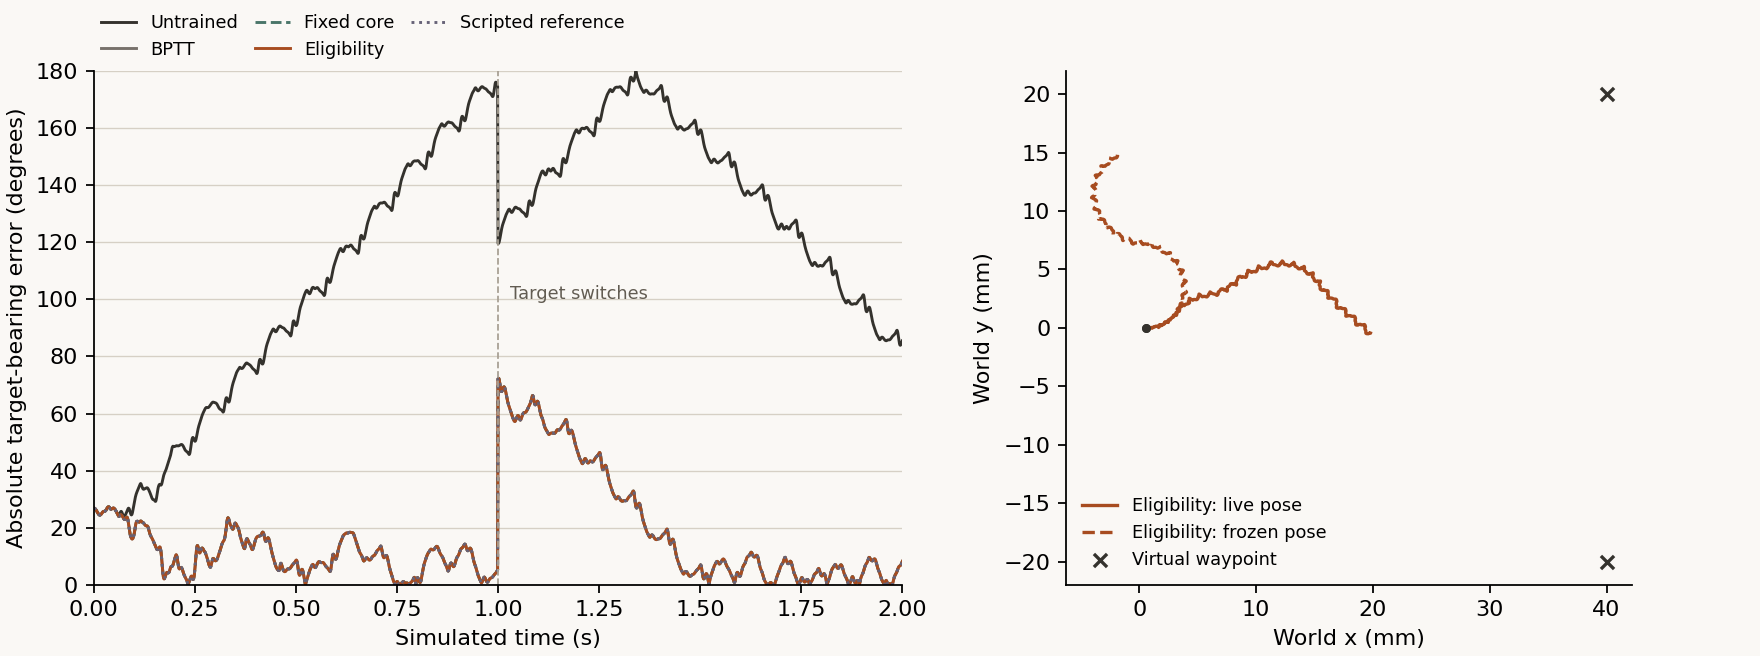
\includegraphics[width=\linewidth]{closed-loop-switch.png}
\caption{Target-switch scenario. Left: all five live-pose error curves;
identical trajectories overlap. Right: live and frozen pose for the eligibility
network. The target changes at one simulated second.}
\end{figure}

For the predeclared eligibility/live/switch video trial, mean angular error is
\FeedbackSwitchError{} degrees and final target distance is
\FeedbackSwitchDistance{} mm. Distance progress is \FeedbackPhaseOne{} mm in
the first phase and \FeedbackPhaseTwo{} mm in the second. Each phase uses its
own fixed target for both endpoint distances, avoiding an artificial progress
jump when the target switches.

\begin{figure}[h]
\centering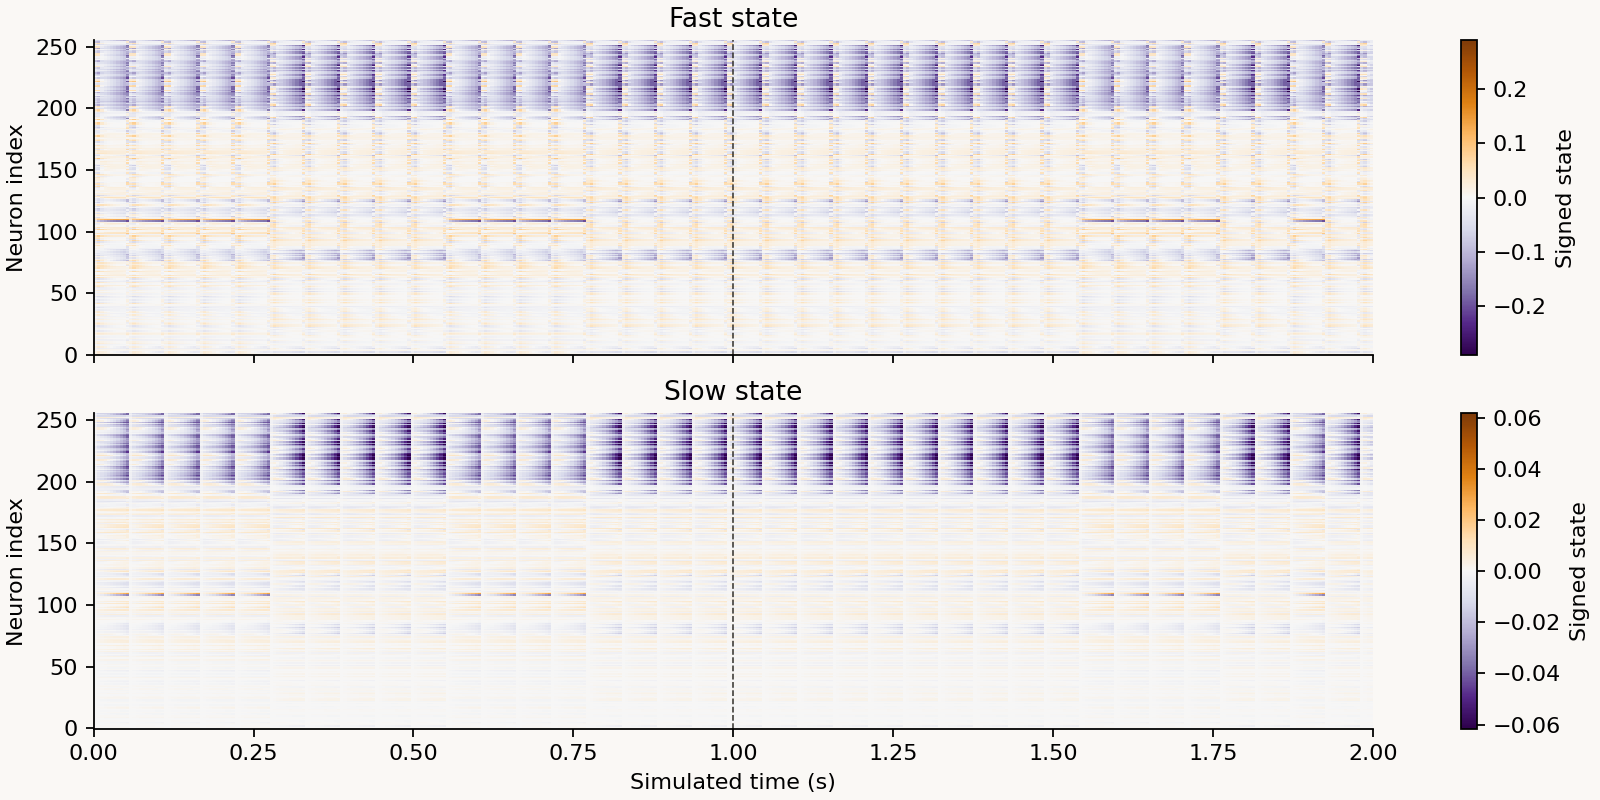
\includegraphics[width=.96\linewidth]{closed-loop-neural.png}
\caption{Actual 256-neuron state during that trial. Each column holds the
inference state for the following 5 ms interval. Separate signed color scales
show fast and slow variables. Eleven-frame resets match the trained episode
interface; these panels do not establish continuous long-term memory.}
\end{figure}

The video contains 200 frames at 25 fps, displaying two simulated seconds in
eight seconds. Its tracking camera follows the body; virtual target coordinates
are shown in the trajectory plot. The repeated trial reproduces every physical
and neural array and all delayed decisions exactly in the recorded environment.

\newpage
\section{Independent verification and reproduction}
The NumPy bridge exports the effective normalized recurrence, time constants,
input projection, pooling, LayerNorm and readout from the original PyTorch
checkpoints. Four fixed 128-frame fixtures include random sensory inputs,
resets and the original zero-distractor cue episodes. Fast/slow state and logits
pass combined absolute tolerance $2\times10^{-6}$ and relative tolerance
$2\times10^{-5}$ in both environments; argmax choices agree. This is numerical
parity within tolerance, not bitwise equivalence between all arithmetic kernels.

The independent auditor recomputes pose-derived sensory inputs and replays all
400 control frames and 36 delayed decisions per condition. It reconstructs the
applied motor timeline and recomputes all reported physical measurements.
The main cohort contains 54,027 body observations, 10,800 control frames and
972 decisions; the separate repeat adds 2,001 observations, 400 frames and
36 decisions. Scripted control frames contain sensory and command records only.

Five fault-injection checks alter cue, query timing, neural state, sampled pose
or phase progress. Each edited archive has a refreshed valid hash; the auditor
still rejects its causal or numerical inconsistency. Complete-cohort reporting
refuses to publish a comparison until all conditions and the repeat pass.

The public records archive includes every NPZ/CSV/JSON record, four controllers,
parity fixtures, source files, graph identities, protocols, licenses and a
payload hash manifest. From a fresh extraction, run
\code{python scripts/audit_feedback_release.py}. Auditing saved records needs
NumPy, without PyTorch or MuJoCo. Fresh physics additionally uses the pinned
FlyGym 2.1.0/MuJoCo 3.9.0 environment and the documented empty-directory workflow;
its identity must remain distinct from the published observations.

\section{What the assay establishes}
The sensory mapping can be exercised in a causal body-feedback loop. The
trained-controller/scripted trajectory comparisons reveal when the engineered
interface makes different internal models behaviorally indistinguishable.
Matching the fixed-core or scripted reference provides no evidence that
trained recurrent dynamics were necessary for this task.

The conditions were declared before physical execution, but methods were chosen
from previously observed cue-learning results. The experiment is exploratory.
Ground-truth position, sign encoding, an externally prescribed target, episodic
resets, a straight-ahead gate and a designed gait controller all simplify the
problem. The single seed cannot support population claims. No model learns from
physical reward, controls individual joints through learned weights, or transfers
language knowledge to behavior here.

Anatomical utility remains a separate hypothesis requiring matched retrained
wiring controls. The ongoing WikiText study has priority over larger-corpus
training. A later language-to-control study needs an explicit shared interface
and matched adaptation of untrained and language-trained cores; this physical
assay cannot substitute for that comparison.

\bibliographystyle{plain}
\bibliography{references}
\end{document}
